\documentclass[tikz,border=6pt]{standalone}
\usepackage{pgfplots}
\pgfplotsset{compat=1.18}
\begin{document}
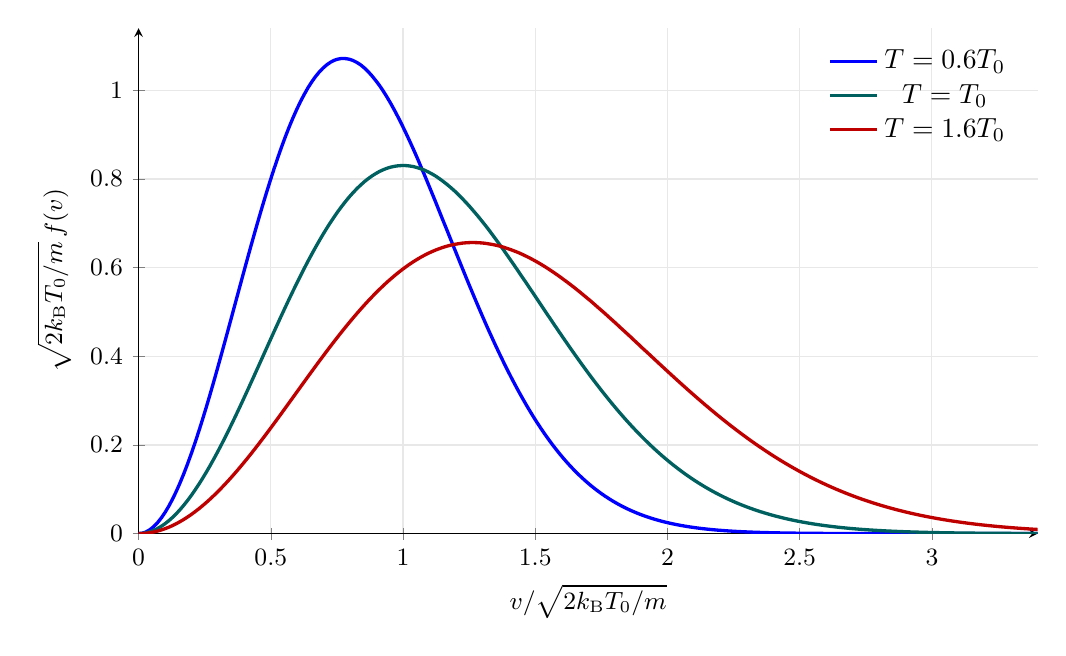
\begin{tikzpicture}
\begin{axis}[
  width=13cm,height=8cm,
  axis lines=left,
  xlabel={$v/\sqrt{2k_{\mathrm B}T_0/m}$},
  ylabel={$\sqrt{2k_{\mathrm B}T_0/m}\,f(v)$},
  xmin=0,xmax=3.4,ymin=0,ymax=1.14,
  samples=240,domain=0:3.4,
  legend style={draw=none,fill=none,at={(0.98,0.98)},anchor=north east},
  tick label style={font=\small},label style={font=\small},
  grid=major,grid style={gray!18}
]
% With x=v/sqrt(2 k_B T0/m), the normalized density is
% f_x=4 x^2 exp(-x^2/tau)/(sqrt(pi) tau^(3/2)), tau=T/T0.
\addplot[very thick,blue] {4*x^2*exp(-x^2/0.6)/(sqrt(pi)*0.6^(3/2))};
\addlegendentry{$T=0.6T_0$}
\addplot[very thick,teal!75!black] {4*x^2*exp(-x^2)/(sqrt(pi))};
\addlegendentry{$T=T_0$}
\addplot[very thick,red!75!black] {4*x^2*exp(-x^2/1.6)/(sqrt(pi)*1.6^(3/2))};
\addlegendentry{$T=1.6T_0$}
\end{axis}
\end{tikzpicture}
\end{document}
